\section{Theorie}
\label{sec:Theorie}

Betrachtet wird in diesem Versuch das Verhalten elektrischer Signale auf Leitern. Hierbei wird zuerst der Aufbau einer verlustfreien und verlustbehafteten Schaltung in folgender Abbildung betrachtet.
\begin{figure}[H]
    \centering
    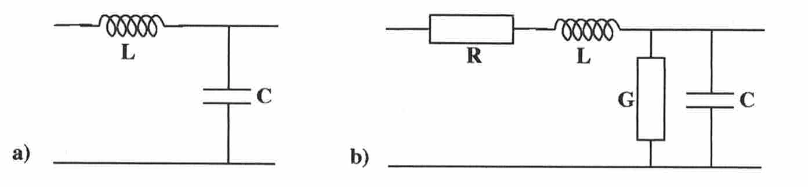
\includegraphics[width=0.8\textwidth]{content/pics/schaltung.png}
    \caption{Verlustfreie und verlustbehaftete Schaltung.}
    \label{fig:Schaltung}
\end{figure}
Zunächst werden die Leitungskonstanten $R, L, C$ und $G$ definiert. Hierbei ist $R$ der Widerstand pro Längeneinheit, $L$ die Induktivität pro Längeneinheit, $C$ die Kapazität pro Längeneinheit und $G$ die Leitfähigkeit pro Längeneinheit.
Bei $R$ dem ohmschen Widerstand wird elektrische Energie in Wärme umgewandelt, bei $L$ der Induktivität wird elektrische Energie in magnetische Energie umgewandelt, bei $C$ der Kapazität wird elektrische Energie in elektrische Energie umgewandelt und bei $G$ der Leitfähigkeit wird elektrische Energie in Wärme umgewandelt.
Hierbei wird als Leitung ein Koaxialkabel betrachtet. Dieses besteht aus zwei zylinderförmigen Leitern, welche durch ein Dielektrikum getrennt sind. 
\begin{figure}[H]
    \centering
    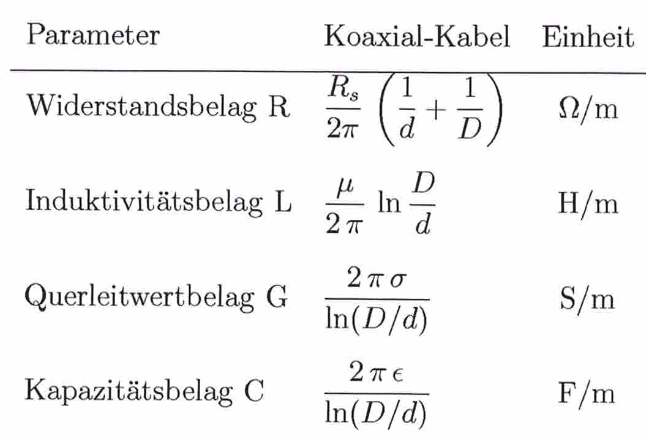
\includegraphics[width=0.4\textwidth]{content/pics/tabelle.png}
    \caption{Formeln zur Bestimmung der Parameter der Leitungsbeläge.}
    \label{fig:tabelle}
\end{figure}
$R_s = \sqrt{\frac{\pi \nu \mu_c}{\sigma_c}}$ ist hierbei eine Konstante, $d$ und $D$ sind Innen- bzw Außenradius des Kabels, $\sigma$ ist die elektrische Leitfähigkeit, $\mu$ ist die magnetische Permeabilität und $\epsilon$ die Dielektrizitätskonstante.  
Um zu beschreiben, wie sich ein Signal auf einer Leitung in Form von Wellen ausbreitet, wird die Telegraphengleichung verwendet. Diese lautet:
\begin{equation*}
\frac{\partial^{2} U}{\partial t^{2}} = L C \frac{\partial^{2} U}{\partial t^{2}} + (LG + RC) \frac{\partial U}{\partial t} + RGU
\end{equation*}
Hierbei ist $U$ die Spannung auf der Leitung.
Die Lösungen der Telegraphengleichung wird durch 
\begin{equation*}
U(z,t) = U e^{-\gamma z} e^{i\omega t}
\end{equation*}
beschrieben. Hierbei ist $z$ die Position auf der Leitung, $\omega$ die Kreisfrequenz und $\gamma$ die Ausbreitungskonstante. Diese wird durch
$\gamma = \alpha + j\beta = \sqrt{(R + j\omega L)(G + j\omega C)}$ beschrieben. Hierbei ist $\alpha$ die Dämpfungskonstante und $\beta$ der Phasenbelag.
Dabei ist $\alpha$ definiert durch:
\begin{equation}
    \alpha = \frac{1}{z} \ln\left(\frac{U_0}{U(z)}\right)
\end{equation}
Für die Geschwindikeit der Signale gilt $v = \frac{c_0}{\sqrt{\epsilon_r}}$, da sich die elektromagnetischen Wellen mit Lichtgeschwindigkeit ausbreiten, hierbei ist $c_0$ die Lichtgeschwindigkeit und $\epsilon_r$ die relative Dielektrizitätskonstante.
Diese 
Eine verlustbehaftete Leitung führt zur Verzerrung des Signals.
Der Wellenwiderstand $Z_0$ einer Leitung wird durch 
\begin{equation*}
Z_0 = \frac{U(\omega)}{I(\omega)} = \sqrt{\frac{R + j\omega L}{G + j\omega C}}
\end{equation*}
beschrieben. 
Des Weiteren ist zu beschreiben, wie sich $Z$ berechnen lässt 
\begin{align}
    Z &= R + i\omega L \\
    \left| Z \right| &= \sqrt{R^2+\omega^2 L^2}\\
    \tan(\phi) &= \frac{\omega L}{R}
\end{align}
$\phi$ ist die Phasenverschiebung und $\omega$ die Kreisfrequenz.
Mit folgender Schaltung 
\begin{figure}[H]
    \centering
    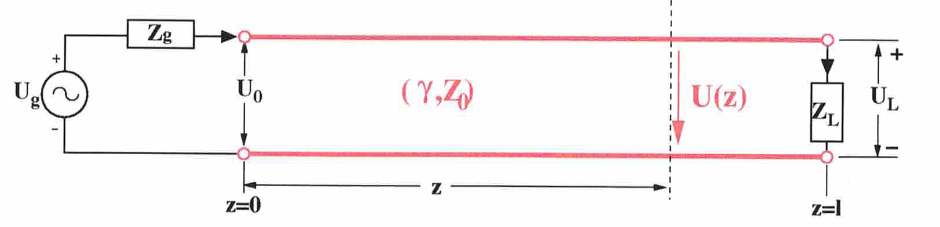
\includegraphics[width=0.8\textwidth]{content/pics/abschluss.png}
    \caption{Schaltung einer Leitung mit einem Funktionsgenerator und einem Abschlusswiderstand.}
    \label{fig:Leitung}
\end{figure}
kann das Verhalten elektrischer Signale auf Leitern untersucht werden. Hierbei wird ein Signal von einem Funktionsgenerator eingespeist und die Spannung am Ende der Leitung mit einem Oszilloskop gemessen. Je nach Abschlusswiderstand $Z_L$ kann es zu Reflexionen kommen, welche durch den Reflexionsfaktor $\Gamma$ beschrieben werden. Dieser wird durch
\begin{equation*}
\Gamma = \frac{U_{r}}{U_{0}} = \frac{Z_{L} - Z_{0}}{Z_{L} + Z_{0}} = |\Gamma| e^{i\varphi_{\Gamma}}
\end{equation*}
beschrieben. Hierbei ist $U_r$ die reflektierte Spannung, $U_0$ die eingehende Spannung, $Z_L$ der Abschlusswiderstand und $Z_0$ der Wellenwiderstand der Leitung. 
In der folgenden Abilldung werden beispielsweise die Signalverläufe für verschiedene Abschlusswiderstände dargestellt.
\begin{figure}[H]
    \centering
    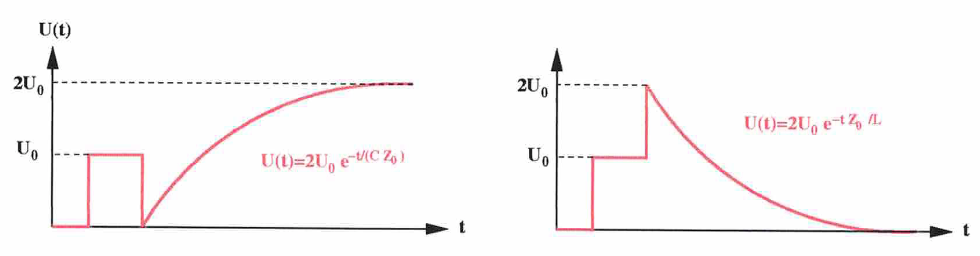
\includegraphics[width=0.8\textwidth]{content/pics/verschiedenabschluss.png}
    \caption{Signalverläufe für einen Kondensator(links) und eine Spule(rechts) als Abschlusswiderstand.}
    \label{fig:Abschlussverlaeufe}
\end{figure}

\clearpage